\documentclass{standalone}
\usepackage{tikz}
\usetikzlibrary{calc}
\usepackage{hsbcommon}
  

\begin{document}
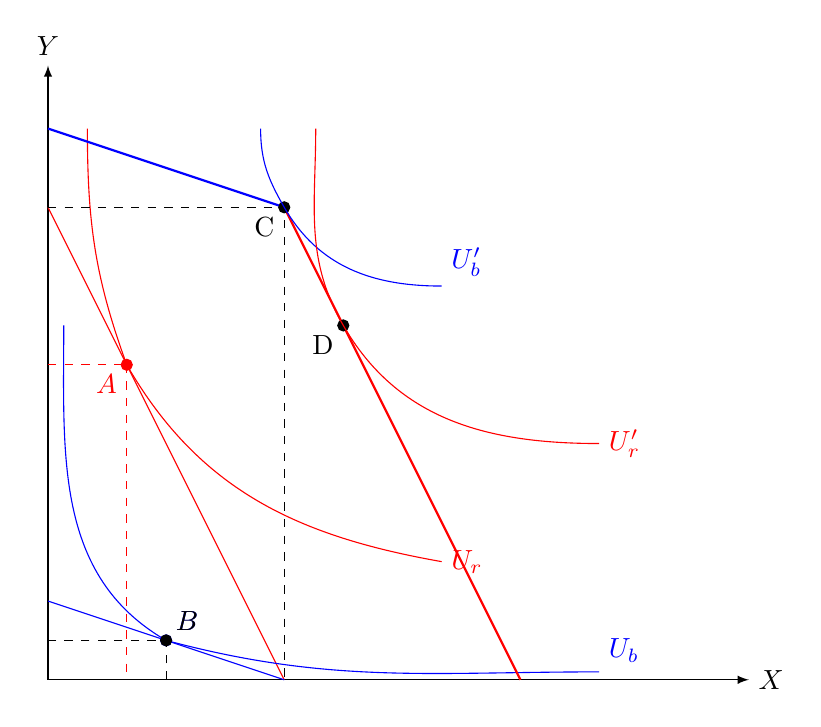
\begin{tikzpicture}% [scale=0.6]
    %Axis
    \draw [<-,>=latex] (0,7.8) node [above] {$Y$} -- (0,0);
    \draw[->,>=latex] (0,0) -- (8.9,0) node [right] {$X$};

    % Production frontiers
    
    
    % Red

    \ifstep{1}{
\begin{scope}[color=red]

        
    \draw(0,6) -- (3,0);
    
    \coordinate (rx) at (1,4);
        \draw[red] (0.5,7) 
            to [out=-90, in=110] (rx) 
            to [out=-60, in=170] (5,1.5) node[right] {$U_r$};
            ;
        \draw[red,dashed] (0,4) -- (rx);
        \draw[red,dashed] (rx) -- (1,0);

        \filldraw (rx) circle (2pt) node[below left] {$A$};

    % \draw[black,ultra thick] (0,3) -- (3,0);

    \end{scope}
}

    \ifstep{2}{
\begin{scope}[color=blue]

        
        \draw (0,1) -- (3,0);
        \coordinate (bx) at (1.5,0.5);
        \draw  (7,0.1)  node[above right] {$U_b$}
            to [in=-15, out=180] (bx) 
            to [out=150, in=-90] (0.2,4.5)
            ;
        \draw[dashed] (bx |-, 0) -- (bx) -- (0, |- bx);

        \filldraw (bx) circle (2pt) node[above right] {$B$};
        
    \end{scope}
}

    \ifstep{3}{
\begin{scope}[color=black]

        \draw[blue,thick] (0,7) -- (3,6);
        \draw[red,thick] (3,6) -- (6,0);
        \coordinate (cx) at (3,6);
        \filldraw (cx) circle (2pt) node[below left] {C};
        \draw[dashed] (0, |- cx) -- (cx) -- (cx |-,0);
        
        \draw[blue]  (5,5)  node[above right] {$U'_b$}
            to [in=-60, out=180] (cx) 
            to [out=120, in=-90] (2.7,7)
            ;
        
        \coordinate (L) at (3,6);
        \coordinate (K) at (6,0);
        \coordinate (dx) at ($(L)!0.25!(K)$);

        \filldraw (dx) circle (2pt) node[below left] {D};
        \draw[red]  (7,3)  node[right] {$U'_r$}
            to [in=-60, out=180] (dx) 
            to [out=120, in=-90] (3.4,7)
            ;
        \draw[dashed] (bx |-, 0) -- (bx) -- (0, |- bx);

        \filldraw (bx) circle (2pt) node[above right] {$B$};

        
    \end{scope}
}

    % \ifstep{3}{

        
    %     \coordinate (sx) at (3,3);
    %         \draw (7,2)  node[right] {$U_{\text{trade}}$}
    %             to [in=-30, out=175] (sx) 
    %             to [out=130, in=-85] (2,7)
    %             ;
    %         \draw[dashed] (3,0) -- (sx);
    %         \draw[dashed] (sx) -- (0,3);
    
    %     \filldraw (sx) circle (2pt) node[above right] {$T$};
    %     \draw[black,thick] (0,6) -- (6,0) ;
    % }

    

\end{tikzpicture}
\end{document}
